\documentclass{article}
\usepackage[top=1in, bottom=1in, left=1in, right=1in]{geometry}
\usepackage{graphicx}
\begin{document}

\begin{flushright}
Matt Jibson \\
EG 510 \\
HW 11
\end{flushright}

\begin{enumerate}
	\item
		\begin{itemize}
			\item [(a)] Graphical solution: $x_1 = 0, x_2 = 4, -x_1 - x_2 = -4$: \\
				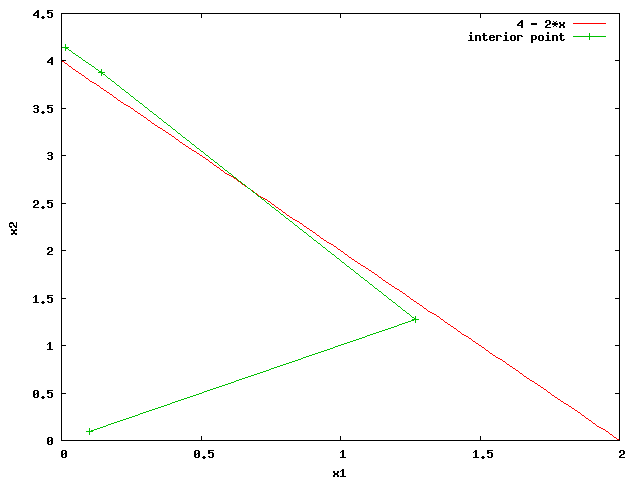
\includegraphics[width=0.8\linewidth]{1a.png}
			\item [(b)]
				\begin{displaymath}
					\mathbf{x}_0 = \left[ \begin{array}{c} 0.1 \\ 0.1 \\ 3.7 \end{array} \right],
					\mathbf{D} = \left[ \begin{array}{c c c} 0.1 & 0 & 0 \\ 0 & 0.1 & 0 \\ 0 & 0 & 3.7 \end{array} \right],
					\mathbf{B} = \mathbf{AD} = \left[ \begin{array}{c c c} 0.2 & 0.1 & 3.7 \end{array} \right],
				\end{displaymath}
				\begin{displaymath}
					\mathbf{BB}^T = \left[ \begin{array}{c} 13.74 \end{array} \right], \mathbf{Dc} = \left[ \begin{array}{c} -0.1 \\ -0.1 \\ 0 \end{array} \right], \mathbf{BDc} = \left[ \begin{array}{c} -0.03 \end{array} \right],
				\end{displaymath}
				\begin{displaymath}
					\mathbf{w} = \left[ \begin{array}{c} -0.02183 \end{array} \right], \mathbf{c}_p = \left[ \begin{array}{r} 0.0996 \\ 0.0998 \\ -0.008079 \end{array} \right], \theta = 1/0.008079 = 123.778, \alpha = 0.9 \Rightarrow
				\end{displaymath}

				\begin{displaymath}
					\mathbf{x}_1 = \left[ \begin{array}{c} 1.209 \\ 1.212 \\ 0.37 \end{array} \right],
					\mathbf{D} = \left[ \begin{array}{c c c} 1.209 & 0 & 0 \\ 0 & 1.212 & 0 \\ 0 & 0 & 0.37 \end{array} \right],
					\mathbf{B} = \mathbf{AD} = \left[ \begin{array}{c c c} 2.418 & 1.212 & 0.37 \end{array} \right],
				\end{displaymath}
				\begin{displaymath}
					\mathbf{BB}^T = \left[ \begin{array}{c} 7.453 \end{array} \right], \mathbf{Dc} = \left[ \begin{array}{c} -1.209 \\ -1.212 \\ 0 \end{array} \right], \mathbf{BDc} = \left[ \begin{array}{c} -4.392 \end{array} \right],
				\end{displaymath}
				\begin{displaymath}
					\mathbf{w} = \left[ \begin{array}{c} -0.5894 \end{array} \right], \mathbf{c}_p = \left[ \begin{array}{r} -0.2161 \\ 0.4977 \\ -0.2181 \end{array} \right], \theta = 1/0.2181 = 4.585, \alpha = 0.9 \Rightarrow
				\end{displaymath}

				\begin{displaymath}
					\mathbf{x}_2 = \left[ \begin{array}{c} 0.1311 \\ 3.7 \\ 0.037 \end{array} \right],
					\mathbf{D} = \left[ \begin{array}{c c c} 0.1311 & 0 & 0 \\ 0 & 3.7 & 0 \\ 0 & 0 & 0.037 \end{array} \right],
					\mathbf{B} = \mathbf{AD} = \left[ \begin{array}{c c c} 0.2622 & 3.7 & 0.037 \end{array} \right],
				\end{displaymath}
				\begin{displaymath}
					\mathbf{BB}^T = \left[ \begin{array}{c} 13.76 \end{array} \right], \mathbf{Dc} = \left[ \begin{array}{c} -0.1311 \\ -3.7 \\ 0 \end{array} \right], \mathbf{BDc} = \left[ \begin{array}{c} -13.724 \end{array} \right],
				\end{displaymath}
				\begin{displaymath}
					\mathbf{w} = \left[ \begin{array}{c} -0.9974 \end{array} \right], \mathbf{c}_p = \left[ \begin{array}{r} -0.1304 \\ 0.0096 \\ -0.0369 \end{array} \right], \theta = 1/0.1304 = 7.6687, \alpha = 0.9 \Rightarrow
				\end{displaymath}

				\begin{displaymath}
					\mathbf{x}_3 = \left[ \begin{array}{c} 0.0131 \\ 3.946 \\ 0.0278 \end{array} \right]
				\end{displaymath}

			\item [(d)] Dual is: \\
				\begin{displaymath}
					\begin{array}{ll}
					\textrm{maximize} & w = 4y_1 \\
					\textrm{subject to} & 2y_1 \le -1 \\
					& y_1 \le -1 \\
					& y_1 \le 0 \\
					& y_1 \; \mathrm{free}
					\end{array}
				\end{displaymath}

				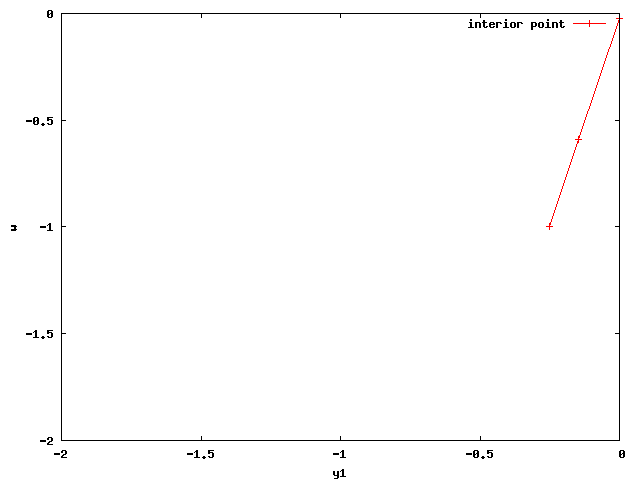
\includegraphics[width=0.7\linewidth]{1d.png}

				The feasible range is $y_1 \le -1$, and the \textbf{w}'s generated in the affine scaling alrorithm are converging on the dual solution of $y_1 = -1$.
		\end{itemize}

	\item Original problem:
		\begin{displaymath}
			\begin{array}{ll}
			\textrm{minimize} & -x_1 - x_2 \\
			\textrm{subject to} & 2x_1 + x_2 + x_3 = 1 \\
			& x_i \ge 0
			\end{array}
		\end{displaymath}
		Phase I problem:
		\begin{displaymath}
			\begin{array}{ll}
			\textrm{minimize} & \lambda \\
			\textrm{subject to} & 2x_1 + x_2 + x_3 + 3 \lambda = 1 \\
			& \lambda \ge 0, x_i \ge 0
			\end{array}
		\end{displaymath}
		Set $x_i, \lambda = 1$:
			\begin{displaymath}
				\mathbf{x}_0 = \left[ \begin{array}{c} 1 \\ 1 \\ 1 \\ 1 \end{array} \right],
				\mathbf{D} = \left[ \begin{array}{c c c c} 1 & 0 & 0 & 0 \\ 0 & 1 & 0 & 0 \\ 0 & 0 & 1 & 0 \\ 0 & 0 & 0 & 1 \end{array} \right],
				\mathbf{B} = \mathbf{AD} = \left[ \begin{array}{c c c c} 2 & 1 & 1 & 3 \end{array} \right],
			\end{displaymath}
			\begin{displaymath}
				\mathbf{BB}^T = \left[ \begin{array}{c} 15 \end{array} \right], \mathbf{Dc} = \left[ \begin{array}{c} 0 \\ 0 \\ 0 \\ 1 \end{array} \right], \mathbf{BDc} = \left[ \begin{array}{c} 3 \end{array} \right],
			\end{displaymath}
			\begin{displaymath}
				\mathbf{w} = \left[ \begin{array}{c} 0.2 \end{array} \right], \mathbf{c}_p = \left[ \begin{array}{r} 0.4 \\ 0.2 \\ 0.2 \\ -0.4 \end{array} \right], \theta = 1/0.4 = 2.5, \alpha = 1 \Rightarrow
			\end{displaymath}
			\begin{displaymath}
				\mathbf{x}_1 = \left[ \begin{array}{c} 2 \\ 1.5 \\ 1.5 \\ 0 \end{array} \right]
			\end{displaymath}
\end{enumerate}

\end{document}
